\begin{mainquestion}{nodalreference}{Nodal Analysis I}

\questionpoints Steel yourself for some math! You will use nodal analysis to determine the voltage across each (non-voltage source) element and the currents $i_{2}$ through $i_{8}$.

\begin{center}
    % [width=0.8\textwidth] makes the image take up 80% of the text width
    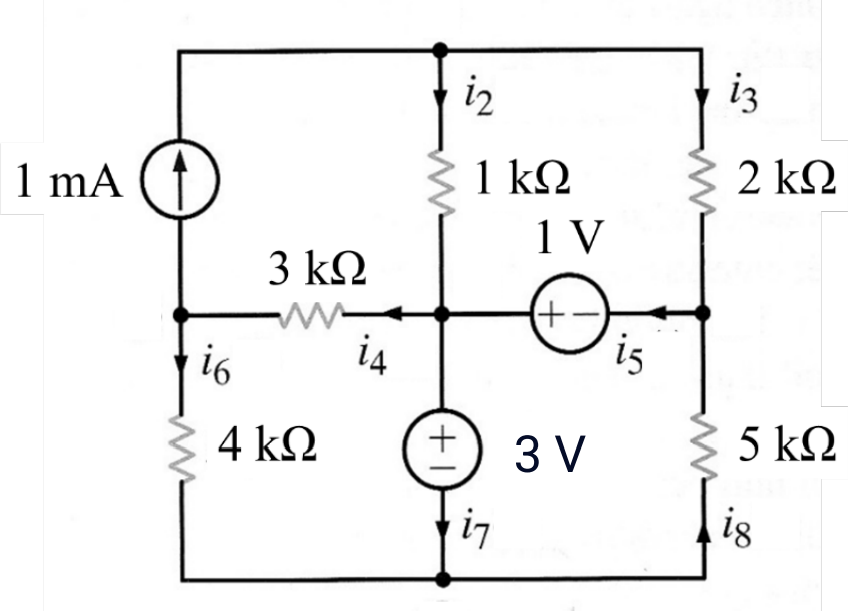
\includegraphics[width=0.5\textwidth]{nodal_analysis.png}
\end{center}

% =========================================================
\begin{partquestion}{referencenode}
{Choose an appropriate node to be the reference (ground). How many unknown node voltages remain after choosing the reference node? Clearly state which node voltages are unknown.}

\begin{answer}[2in]
\end{answer}

\end{partquestion}

% =========================================================
\begin{partquestion}{kclequations}
{Using nodal analysis, write the KCL equations for each node with an unknown voltage. Express each equation in terms of the labeled branch currents, and then express these branch currents in terms of the node voltages.}

\begin{answer}[2.5in]
\end{answer}

\end{partquestion}

% =========================================================
\begin{partquestion}{solvenodes}
{Solve the nodal equations to determine the numerical values of the unknown node voltages.}

\begin{answer}[3in]
\end{answer}

\end{partquestion}

% =========================================================
\begin{partquestion}{branchcurrents}
{Using the node voltages found in part (d), compute the values of the unknown branch currents $i_{2}$ through $i_{8}$. Indicate the sign of each current relative to the directions shown in the circuit.}

\begin{answer}[2in]
\end{answer}

\end{partquestion}

\end{mainquestion}
